%Results

\subsubsection*{Division of labour}
Our model is able to simulate the divison of labour. In Fig.\ref{fig:thetax} on the left we see the development of the thresholds $\theta_{ij}$ as a function of time. For each individuum $i$ there is one line with respect to each task $j$. Here, we have used N=5 bees and M=2 tasks, amounting to 10 depicted lines - one line for each task for each bee. We can see that in the beginning the values of $\theta_{ij}$ oscillate and then assume a steady state from approximately $t=3000$ on. In this steady state, exactly five lines assume the constant maximum value $\theta_{ij}=1000$ and five lines assume the constant minimum value $\theta_{ij}=0$. This means that the five bees specialize in exactly one task and keep performing this single task in the steady state.

\begin{figure}[ht!]
	\centering
	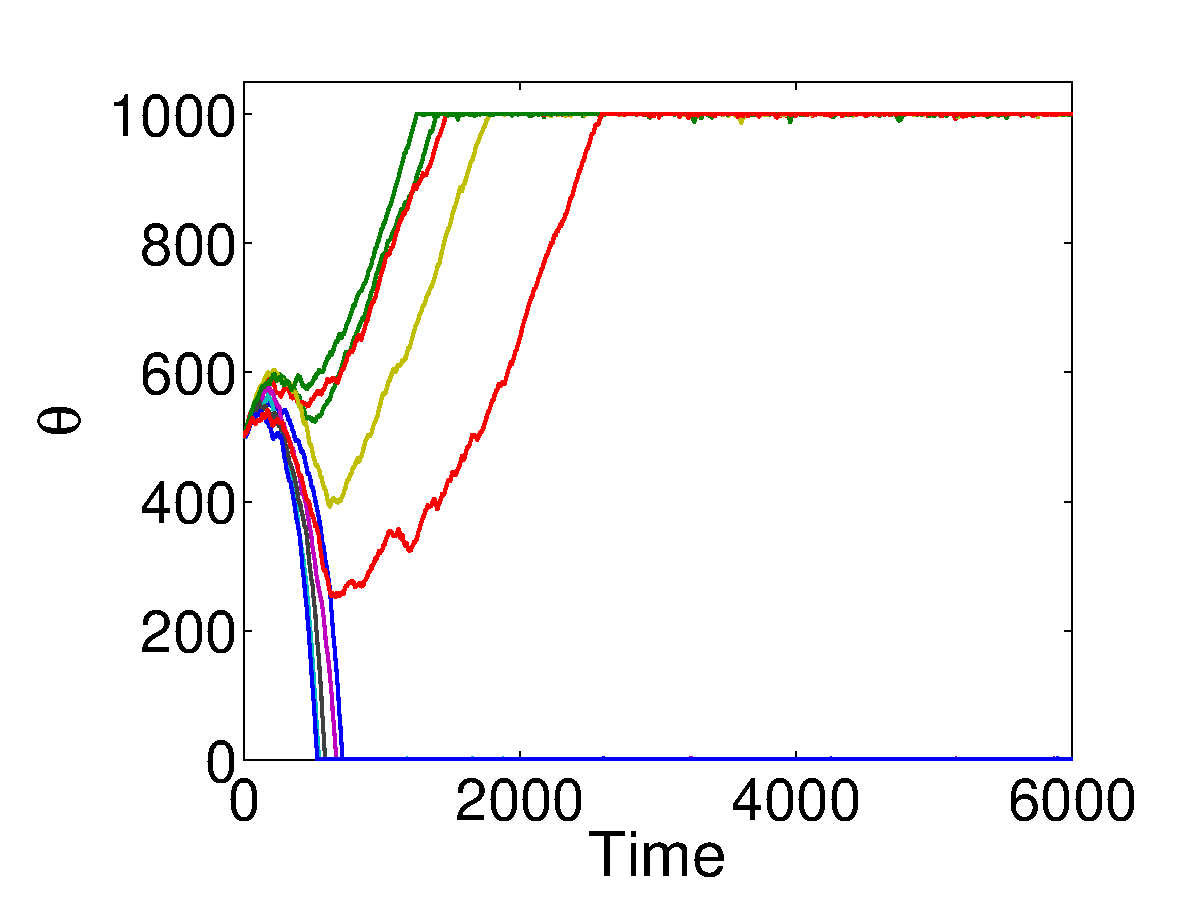
\includegraphics[width=0.4\textwidth]{figures/thetax.eps}
	\caption{$\theta$ as a function of time.}
	\label{fig:thetax}
\end{figure}

This behaviour can be explained as follows. In the beginning, the five bees have no preference for any task as their $\theta=500$ for all tasks. In other words, there is no specialization yet. First, a bee tries out to perform one of the two tasks and gets inactive with a certain probability over time. It might subsequently decide to continue pursuing its first task or alternatively perform the second one. This decision is influenced by two factors. First, by the choice of the other bees. If all bees perform task 1, the stimulus for this task will be negligible compared to the increasing stimulus for task 2 and it becomes more likely to perform this second task. Second, by the skills the bee has gained or forgotten with respect to a specific task. The more time a bee spends pursuing task 1, the better it gets performing it. In our model, the bee is then more likely to continue pursuing this task. Vice versa is true for a task which is not performed regularly by a bee. Therefore, what we observe is that some bees will exclusively perform task 1, thus $\theta_{j=1}=0$ and $\theta_{j=2}=1000$ in the steady state, and others decide to perform task 2, thus $\theta_{j=2}=0$ and $\theta_{j=1}=1000$. The model consequently allows for the investigation of the division of labour in societies. Driving force for the division is the specialization by a learning and forgetting process.
In Fig.\ref{fig:thetax}  on the right we can see x as a function of time.

\subsubsection*{Measurement of the development and performance of a society}
Our model enables the description of the performance of the bee hive. In Fig.\ref{fig:welstim} the thresholds, the corresponding stimuli with respect to task $j=1, 2$ as well as the corresponding total welfare W of the society is depicted. The behaviour of the thresholds is analogous to what is already described in Fig.\ref{fig:thetax}. The corresponding stimuli increase in time, reach a maximum value at approximately time=500 and subsequently decrease to zero. Remarkably, the stimulus of task 2 decreases slower than that of task 1. The development of the welfare curve is closely related to the development of the stimuli. At times the stimuli are high the welfare is low. Thus, the welfare first decreases, goes through a minimum at approximately time=500 and then slowly increases to reach its maximum value of 1. Note that in all graphs all functions reach its steady state value at approximately time=3000.

\begin{figure}[ht!]
	\centerline{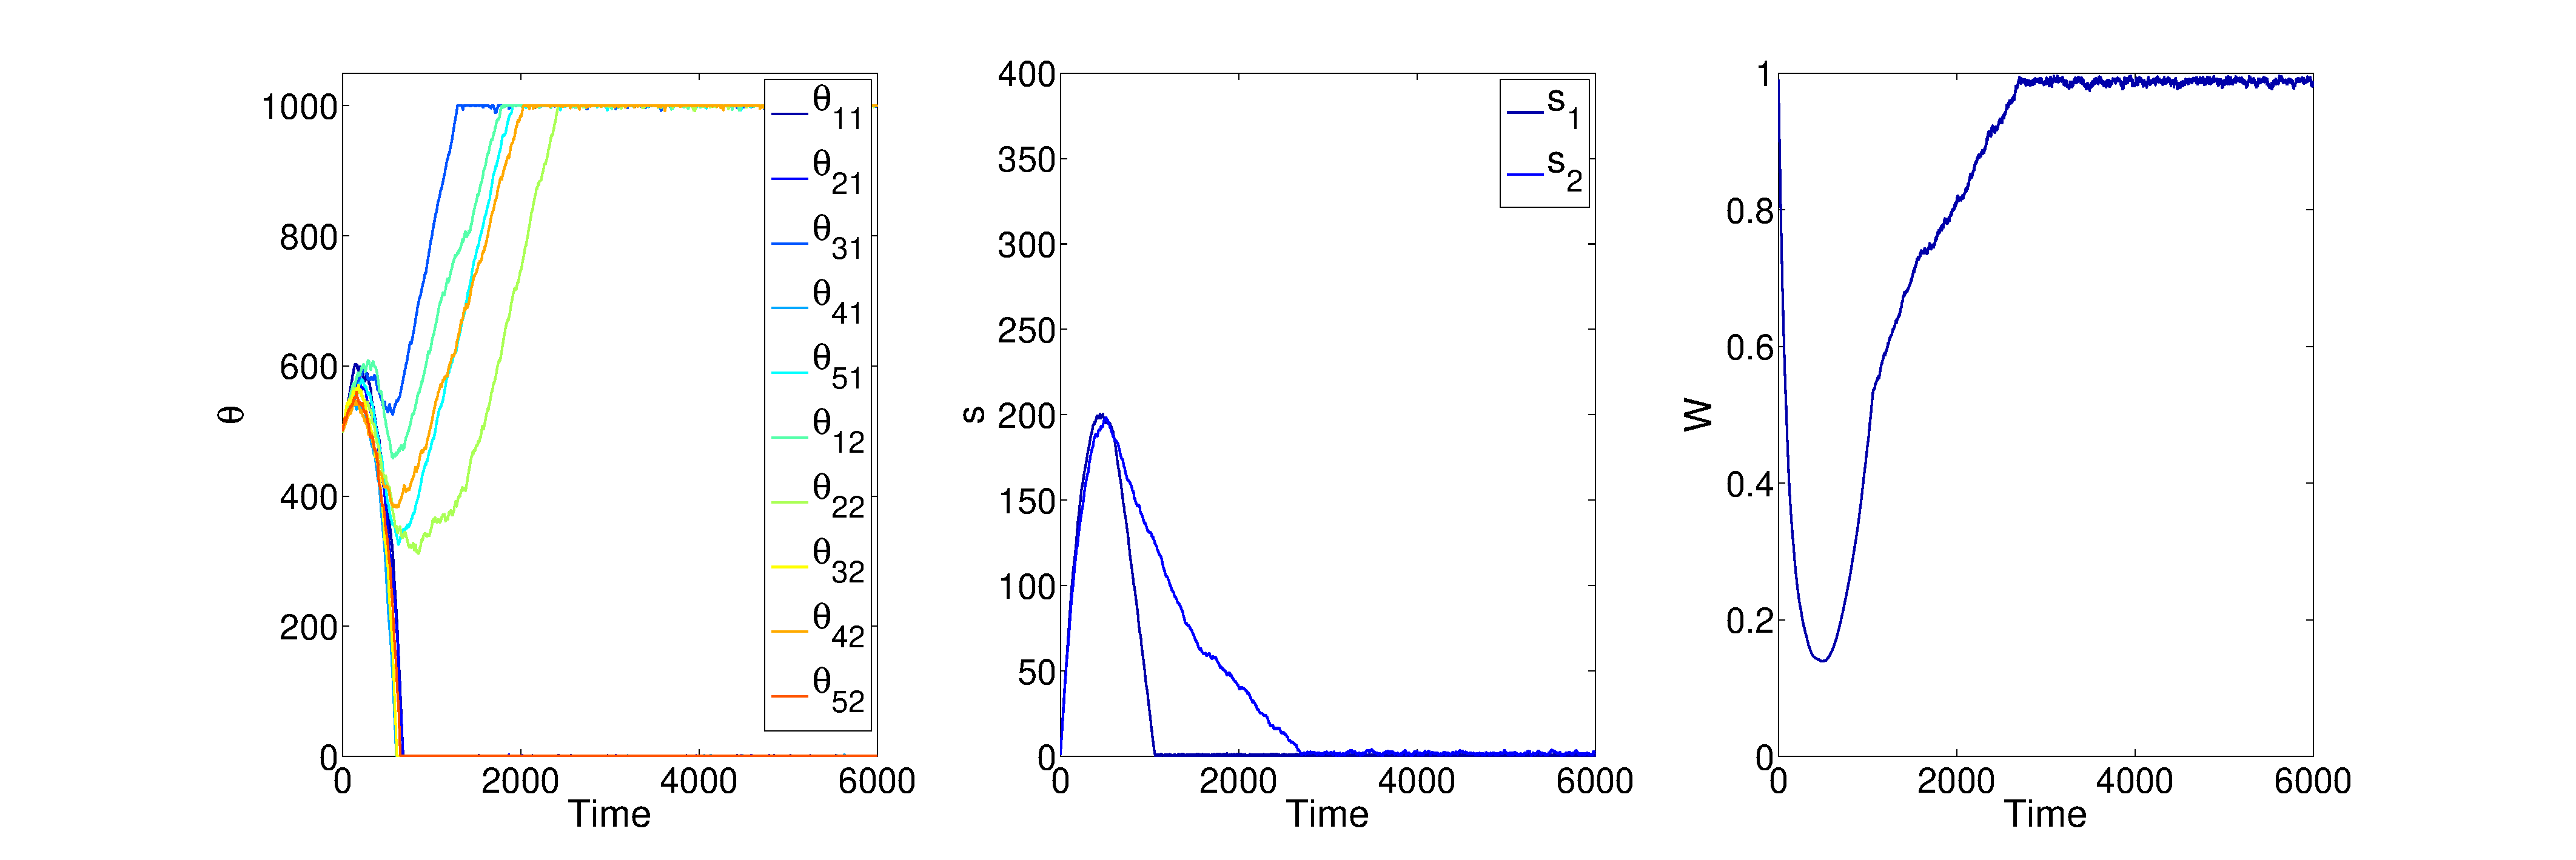
\includegraphics[width=1.25\textwidth]{figures/welstim.eps}}
	
	\caption{Left: Tresholds $\theta$ as a function of time. Middle: Stimuli $s_{j}$ for task 1 and two as a function of time. Right: Welfare W as a function of time.}
	\label{fig:welstim}
\end{figure}

The functions can be interpreted as follows. The development of the stimuli can be explained by the fact that it takes time for the bees to reach an equilibrium state -- the state where all bees assume exactly one task. Up to this point, the needs of the hive are not sufficiently satisfied. Hence, the stimuli increase. Over time, the bees become more specialized towards a specific task and the stimuli go through a maximum to decrease subsequently. This is an expression that the tasks are performed with a sufficient efficiency. The individual development of the thresholds and stimuli is governed by how fast the bees manage to specialize themselves and satisfy the need for the respective task. In the presented case, for example, one can look at the stimulus and the threshold value which converge last to their equilibrium value - stimulus 2 and threshold $\theta_{22}$. Stimulus 2 decreases slower than stimulus 1, so the need to perform 2 is greater for a longer period of time compared to task 1. This is reflected in the curve of $\theta_{22}$. It remains low as long as stimulus 2 is high and only then converges to 1000. This means that bee 2 engages as long in task 2 as stimulus 2 remains high. Thereafter it becomes inactive with respect to task 2 and is thus the last bee to be fully specialized. The welfare is connected to the sum of the stimuli. The stimuli are high when the hive need that specific tasks need to be performed in order for the hive to survive. Whenever a task is not performed, or to an insufficient extent, the respective stimulus is high. High stimuli thus reflect a poor state. Vice versa, low stimuli show that the hive performs well. Therefore, we have introduced the welfare model which is based on the sum of the stimuli. When the sum of the stimuli is low, indicating a good performance of the hive, the welfare increases. Hence, our model is able to describe how well specific tasks are performed and to measure the total welfare of a population over time.


 

